% ============================================================
%  Time models: asynchronous, synchronous, eventually synchronous
% ============================================================

% Delay-over-time plot used in this section.
% \delayaxes{x_end}{y_threshold}
\newcommand{\delayaxes}[2]{%
  \draw[-{Latex}] (0,0) -- (#1,0) node[below left, font=\scriptsize] {time};
  \draw[-{Latex}] (0,0) -- (0,2.6) node[left, font=\scriptsize] {delay};
  \draw[dashed, BrickRed] (0,#2) -- (#1-0.2,#2) node[above left, font=\scriptsize, text=BrickRed] {threshold};
}

\section{Time models: asynchronous, synchronous and eventually synchronous}

In \Cref{def:timing-models} we have already met the three timing models. In this chapter time becomes the main character, so we start by looking at them again in more detail.

\begin{frameddefn}[label={def:time-models-2}]{Time models}
  \begin{itemize}
    \item \textbf{Asynchronous}: there is no bound on the delay that a message can accumulate. This is the model we have used so far.
    \item \textbf{Synchronous}: there is a \textit{known} bound $\delta$ on the delay that a message can accumulate, i.e. if a message is sent at time $t$, it is received by time $t + \delta$.
    \item \textbf{Eventually synchronous}: there is a time, unknown to us, after which the system will be synchronous.
  \end{itemize}
\end{frameddefn}

\subsection{The asynchronous model}

An asynchronous system is characterized by three features:
\begin{itemize}
  \item \textbf{No global clock}: each process only has a local clock, which can be used to order its own events but says nothing about the events of the other processes.
  \item \textbf{No bound on message delays}: a message can take an arbitrarily long (but finite) time to be delivered.
  \item \textbf{Unpredictable local steps}: the computation steps $\Exec(j)$ happen at unpredictable times, decided by the scheduler.
\end{itemize}

As we saw in the previous chapter, in this model a process can't tell a crashed process from a slow one, and it can't even reconstruct the real execution of the system: different executions are indistinguishable.

\subsection{The synchronous model}

A synchronous system is the opposite:
\begin{itemize}
  \item \textbf{Delays are bounded}: every message is delivered within a known time $\delta$.
  \item \textbf{Clocks can be synchronized}, up to a certain precision: processes can agree on the current time with a bounded error.
  \item \textbf{Local steps are predictable}: we can assume that local execution steps happen at predetermined intervals and that they take a bounded amount of time.
\end{itemize}

These assumptions are what allow the processes to proceed in rounds (see the synchronous executions of the previous chapter) and to detect crashes with timeouts: if an answer doesn't arrive within the bound, the sender has surely crashed.

\subsection{Comparing the two models}

The two models are at the opposite ends of a trade-off between \textit{how realistic} the model is and \textit{how much} we can do in it.

\begin{figure}[H]
  \centering
  \begin{tikzpicture}[
      col/.style={draw=RoyalBlue, rounded corners, minimum width=5.4cm, minimum height=2.2cm, align=center, font=\small},
    ]
    \node[col, fill=BrickRed!8] (a) at (0,0) {\textbf{Asynchronous}\\[4pt]
      \textcolor{ForestGreen!60!black}{$+$ models everything}\\[2pt]
      \textcolor{BrickRed}{$-$ agreement is impossible,}\\
      \textcolor{BrickRed}{and a lot of other things}};
    \node[col, fill=ForestGreen!8] (s) at (6.4,0) {\textbf{Synchronous}\\[4pt]
      \textcolor{ForestGreen!60!black}{$+$ almost everything is possible}\\[2pt]
      \textcolor{BrickRed}{$-$ models only restricted networks}};
    \draw[{Latex}-{Latex}, thick, gray] ([yshift=-0.35cm]a.south) -- node[below, font=\scriptsize] {weaker assumptions \quad vs \quad stronger assumptions} ([yshift=-0.35cm]s.south);
  \end{tikzpicture}
  \caption{The trade-off between the asynchronous and the synchronous model.}
  \label{fig:async-vs-sync}
\end{figure}

\begin{itemize}
  \item The asynchronous model \textbf{models everything}: since it assumes nothing about time, every real system is (at least) an asynchronous system, and an algorithm that works in this model works everywhere. The price is that many fundamental problems become unsolvable: for instance, by the FLP result, \textit{agreement} (consensus) is impossible as soon as a single process may crash.
  \item The synchronous model makes \textbf{almost everything possible}, but it \textbf{models only restricted networks}: think of a small dedicated network with real-time guarantees, where bounds on delays can really be enforced. The Internet is not one of them, and an algorithm that relies on a bound that is violated even once can behave incorrectly.
\end{itemize}

We would like a model in between: realistic enough to describe real networks, but strong enough to solve problems like agreement.

\subsection{The eventually synchronous model}

The key observation is that \textbf{real systems are synchronous most of the time}. Consider the following output of the \texttt{ping} command:

\begin{lstlisting}[numbers=none, basicstyle=\ttfamily\scriptsize, frame=single, keywordstyle=\ttfamily]
$ ping google.com
PING google.com (172.217.21.78): 56 data bytes
64 bytes from 172.217.21.78: icmp_seq=0 ttl=53 time=43.239 ms
64 bytes from 172.217.21.78: icmp_seq=1 ttl=53 time=44.621 ms
64 bytes from 172.217.21.78: icmp_seq=2 ttl=53 time=43.540 ms
...
64 bytes from 172.217.21.78: icmp_seq=17 ttl=53 time=38.378 ms
64 bytes from 172.217.21.78: icmp_seq=18 ttl=53 time=739.609 ms
64 bytes from 172.217.21.78: icmp_seq=19 ttl=53 time=38.159 ms
\end{lstlisting}

Almost every packet takes around $40$ ms, so we would be tempted to assume a bound of, say, $\delta = 100$ ms. But every now and then a packet takes much longer, like the $739$ ms of \texttt{icmp\_seq=18}, because of congestion, a busy router or some other temporary problem. The system behaves synchronously most of the time, with short asynchronous periods in between. We have to formalize this \curlyquotes{most of the time}, and this is the concept of \textbf{partial synchrony}.

\begin{figure}[H]
  \centering
  \begin{tikzpicture}[xscale=1.0, yscale=1.0]
    % async periods (shaded)
    \foreach \a/\b in {1.6/2.6, 4.6/5.4, 7.6/8.6} {
      \fill[BrickRed!10] (\a,0) rectangle (\b,2.4);
    }
    \delayaxes{10}{1.2}
    \draw[thick, RoyalBlue] (0.1,0.6) -- (0.5,0.8) -- (0.9,0.5) -- (1.3,0.7) -- (1.7,1.6) -- (2.1,2.1) -- (2.5,1.5) -- (2.8,0.6)
      -- (3.2,0.8) -- (3.6,0.5) -- (4.0,0.7) -- (4.4,0.6) -- (4.8,1.9) -- (5.2,1.4) -- (5.5,0.7)
      -- (5.9,0.6) -- (6.3,0.8) -- (6.7,0.5) -- (7.1,0.7) -- (7.5,0.6) -- (7.9,1.8) -- (8.3,2.2) -- (8.7,0.8) -- (9.1,0.6) -- (9.6,0.7);
    \foreach \x/\l in {0.8/sync, 2.1/async, 3.6/sync, 5.0/async, 6.5/sync, 8.1/async} {
      \node[font=\scriptsize, gray] at (\x,-0.3) {\l};
    }
  \end{tikzpicture}
  \caption{Message delays over time in a real system. Most of the time the delay is below a threshold (synchronous periods), but sometimes it goes above it (asynchronous periods, shaded).}
  \label{fig:partial-synchrony}
\end{figure}

How should an algorithm deal with this behaviour? The answer depends on the kind of property.
\begin{itemize}
  \item \textbf{Safety properties} (e.g.\ mutual exclusion) must hold \textit{always}, also during the asynchronous periods. Since we never know whether we are in a synchronous or in an asynchronous period, safety must never depend on timing assumptions: if an algorithm relied on a bound $\delta$ to guarantee mutual exclusion, a single slow message during an asynchronous period could put two processes in the critical section at the same time, and this violation can never be repaired.
  \item \textbf{Liveness properties} (e.g.\ no-starvation) can instead \textit{use} the synchronous periods. A liveness property only requires that something good happens eventually: if progress is blocked during an asynchronous period, it can still be made during the next synchronous one.
\end{itemize}

This is the typical design principle of algorithms for real systems: \textbf{always safe, live when the system is synchronous}. To be able to prove liveness, we need a precise model of when the system is synchronous.

\begin{frameddefn}[label={def:eventual-sync}]{Eventually synchronous system}
  A system is eventually synchronous if:
  \begin{itemize}
    \item the system is initially asynchronous;
    \item there is a time $T$, unknown to us, after which the system is synchronous and will be synchronous forever.
  \end{itemize}
\end{frameddefn}

\begin{figure}[H]
  \centering
  \begin{tikzpicture}[xscale=1.0, yscale=1.0]
    \fill[BrickRed!10] (0,0) rectangle (6.0,2.4);
    \fill[ForestGreen!10] (6.0,0) rectangle (9.8,2.4);
    \delayaxes{10}{1.2}
    \draw[thick, RoyalBlue] (0.1,0.7) -- (0.5,1.8) -- (0.9,0.6) -- (1.3,2.2) -- (1.7,0.8) -- (2.1,1.5) -- (2.5,0.5) -- (2.9,0.9)
      -- (3.3,2.0) -- (3.7,0.7) -- (4.1,1.4) -- (4.5,0.6) -- (4.9,1.9) -- (5.3,0.8) -- (5.7,1.3)
      -- (6.1,0.6) -- (6.5,0.8) -- (6.9,0.5) -- (7.3,0.7) -- (7.7,0.6) -- (8.1,0.8) -- (8.5,0.5) -- (8.9,0.7) -- (9.4,0.6);
    \draw[very thick, black] (6.0,0) -- (6.0,2.5) node[above, font=\small] {$T$};
    \node[font=\scriptsize, gray] at (3.0,-0.3) {asynchronous (delays unbounded)};
    \node[font=\scriptsize, gray] at (7.9,-0.3) {synchronous forever};
  \end{tikzpicture}
  \caption{An eventually synchronous system: before the unknown time $T$ the delays can be arbitrary, after $T$ they are always below the threshold.}
  \label{fig:eventual-sync}
\end{figure}

\begin{framedobs}{}
  Real systems don't become synchronous \textit{forever}: \Cref{fig:partial-synchrony} shows that asynchronous periods keep coming back. The definition is a mathematical simplification of \curlyquotes{synchronous periods are long enough}: for an algorithm, a synchronous period that lasts forever is equivalent to one that lasts long enough to complete the protocol. Moreover, since $T$ is unknown, an algorithm can't simply wait until $T$: it must be safe during the asynchronous part, and it must be able to make progress after $T$, whenever it happens.
\end{framedobs}

\subsection{Relationship between the models}

\paragraph{Executions.} Let's compare the sets of executions allowed by the three models.
\begin{itemize}
  \item Every synchronous execution is also an eventually synchronous execution, with $T = 0$.
  \item Every eventually synchronous execution is also an asynchronous execution: the asynchronous model allows any (fair) delay, including delays that happen to become bounded after $T$.
\end{itemize}

\begin{figure}[H]
  \centering
  \begin{subfigure}{0.48\textwidth}
    \centering
    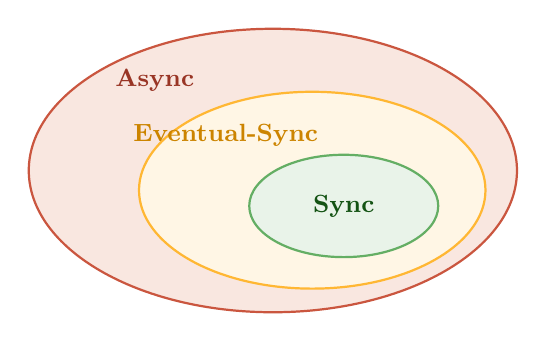
\begin{tikzpicture}
      \draw[thick, BrickRed!70, fill=BrickRed!8] (0,0) ellipse (3.1cm and 1.8cm);
      \draw[thick, Orange!80, fill=Orange!10] (0.5,-0.25) ellipse (2.2cm and 1.25cm);
      \draw[thick, ForestGreen!70, fill=ForestGreen!10] (0.9,-0.45) ellipse (1.2cm and 0.65cm);
      \node[font=\small\bfseries, BrickRed!80!black] at (-1.5,1.15) {Async};
      \node[font=\small\bfseries, Orange!80!black] at (-0.6,0.45) {Eventual-Sync};
      \node[font=\small\bfseries, ForestGreen!60!black] at (0.9,-0.45) {Sync};
    \end{tikzpicture}
    \caption{Relationship between executions.}
  \end{subfigure}
  \hfill
  \begin{subfigure}{0.48\textwidth}
    \centering
    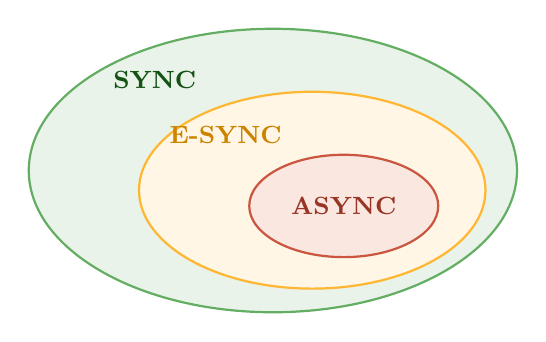
\begin{tikzpicture}
      \draw[thick, ForestGreen!70, fill=ForestGreen!10] (0,0) ellipse (3.1cm and 1.8cm);
      \draw[thick, Orange!80, fill=Orange!10] (0.5,-0.25) ellipse (2.2cm and 1.25cm);
      \draw[thick, BrickRed!70, fill=BrickRed!8] (0.9,-0.45) ellipse (1.2cm and 0.65cm);
      \node[font=\small\bfseries, ForestGreen!60!black] at (-1.5,1.15) {SYNC};
      \node[font=\small\bfseries,  Orange!80!black] at (-0.6,0.45) {E-SYNC};
      \node[font=\small\bfseries, BrickRed!80!black] at (0.9,-0.45) {ASYNC};
    \end{tikzpicture}
    \caption{Relationship of solvable problems.}
  \end{subfigure}
  \caption{The inclusions between the three models are reversed when we go from executions to solvable problems.}
  \label{fig:models-inclusion}
\end{figure}

\paragraph{Solvable problems.} The inclusion is \textit{reversed} for the problems that can be solved. An algorithm for a model must work correctly in \textit{every} execution allowed by that model. The more executions a model allows, the harder it is for an algorithm to handle all of them, and the fewer problems can be solved:
\begin{itemize}
  \item an algorithm that works in the asynchronous model also works in the eventually synchronous one, since it only has to handle a subset of the executions it was designed for; hence every problem solvable in ASYNC is solvable in E-SYNC;
  \item for the same reason, every problem solvable in E-SYNC is solvable in SYNC.
\end{itemize}

\begin{framedex}{Consensus}
  Consensus (agreement) with crash failures shows that the inclusions are strict:
  \begin{itemize}
    \item in SYNC it can be solved for any number of crashes;
    \item in E-SYNC it can be solved if a majority of processes is correct ($f < n/2$), e.g.\ by Paxos, which is always safe and terminates once the system is synchronous;
    \item in ASYNC it can't be solved, even with a single crash (FLP).
  \end{itemize}
\end{framedex}
